%
% Tesi D.S.I. - modello preso da
% Stanford University PhD thesis style -- modifications to the report style
%
%%%%%%%%%%%%%%%%%%%%%%%%%%%%%%%%%%%%%%%%%%%%%%%%%%%%%%%%%%%%%%%%%%%%%%%%%%%
%                                                                         %
%			TESI DOTTORATO                                                   %
%			______________                                                   %
%                                                                         %
%			AUTORE: Elena Pagani                                             %
%                                                                         %
%			Ultima revisione: 7.X.1998                                       %
%           correzioni atrent                                             %
%%%%%%%%%%%%%%%%%%%%%%%%%%%%%%%%%%%%%%%%%%%%%%%%%%%%%%%%%%%%%%%%%%%%%%%%%%%
%
%
\documentclass[a4paper,12pt]{report}
%\renewcommand{\baselinestretch}{1.6}      % interline spacing
%
% \includeonly{}
%
%			PREAMBOLO
%
\usepackage[a4paper]{geometry}
\usepackage{amssymb,amsmath,amsthm}
\usepackage{graphicx}
\graphicspath{ {./images/} }
\usepackage{url}
\usepackage{hyperref}
\usepackage{epsfig}
\usepackage[italian]{babel}
\usepackage{setspace}
\usepackage{tesi}
\usepackage{xcolor}

% per le accentate
\usepackage[utf8]{inputenc}
%
\newtheorem{myteor}{Teorema}[section]
%
\newenvironment{teor}{\begin{myteor}\sl}{\end{myteor}}
%
%
%			TITOLO
%
\begin{document}

\title{Progettazione e sviluppo di test suite automatica e modulo raccolta dati per intelligenze artificiali che si occupano di creare strategie di investimento}
\author{Garion Musetta}
\dept{Corso di Laurea in informatica} 
\anno{2019-2020}
\matricola{920623}
\relatore{Prof. Alfio Ferrara}
\correlatore{Dr. Andrea Bellacicca}
%
%        \submitdate{month year in which submitted to GPO}
%		- date LaTeX'd if omitted
%	\copyrightyear{year degree conferred (next year if submitted in Dec.)}
%		- year LaTeX'd (or next year, in December) if omitted
%	\copyrighttrue or \copyrightfalse
%		- produce or don't produce a copyright page (false by default)
%	\figurespagetrue or \figurespagefalse
%		- produce or don't produce a List of Figures page
%		  (false by default)
%	\tablespagetrue or \tablespagefalse
%		- produce or don't produce a List of Tables page
%		  (false by default)
% 
%			DEDICA
%
\beforepreface
\prefacesection{}
        {\hfill \Large {\sl dedicato a \dots}}
% 
%			PREFAZIONE
%
\prefacesection{Prefazione}

%
%
%			ORGANIZZAZIONE
\section*{Organizzazione della tesi}
\label{organizzazione}
La tesi \`e organizzata come segue:
\begin{itemize}
\item nel Capitolo 1 ....
\end{itemize}
%
%			RINGRAZIAMENTI
%
\prefacesection{Ringraziamenti}

\afterpreface
% 
% 
%			CAPITOLO 1:
%
%


\chapter{Introduzione}
\label{cap1}
Scopo di questo documento è affrontare il tema delle metodologie di test per intelligenze artificiali, descriverne alcune tecniche ed analizzare risultati ottenuti applicandole in uno specifico dominio.
\\~\\
Fra le diverse tipologie di intelligenze artificiali attualmente disponibili vengono considerate quelle di supporto alle decisioni, le quali si adattano particolarmente bene al problema e all'ambito di applicazione. Quando si sviluppa uno strumento di questo tipo è indispensabile porsi delle domande circa la qualità dei risultati prodotti dalla AI, confrontandoli con un modello ottimale di riferimento. Spesso però questo modello non è disponibile oppure è molto difficile da creare, a volte incalcolabile. I risultati ottenuti dovrebbero anche essere paragonati con quelli ottenuti da altre applicazioni preesistenti che operano nel campo in analisi.

\section{Descrizione dell'ambito di riferimento}
Il dominio considerato è quello della finanza, in particolare lo sviluppo di strategie di investimento intelligenti.\\
L'intelligenza artificiale (AI) da testare (\textbf{Sentyment}) genera diverse strategie di investimento personalizzate per numerosi strumenti finanziari ed è anche in grado di piazzare direttamente ordini sul mercato, cioè effettuare operazioni di acquisto e vendita. Il mercato in cui opera è quello delle criptovalute, di queste, Bitcoin è il tipo più famoso ed asset più valevole a livello di borsa valori, insieme ad altre monete come Ethereum, Bitcoin Cash e Ripple, meno famose ma con le loro particolarità e altrettanto scambiate.\\
L'obiettivo finale di Sentyment è produrre delle \textbf{strategie di investimento}, ossia approcci di investimento personalizzati in funzione della propensione al rischio, degli obiettivi e degli interessi specifici del singolo investitore. Seguendo tale strategia, l’investitore può decidere tra diversi tipi di attività da includere nel proprio portafoglio di investimento.\\
Una specifica strategia di investimento può essere determinata da una serie di fattori, tra cui la propensione al rischio e i rendimenti che si vogliono perseguire sugli investimenti, nonché le attività, le regioni e i settori a cui si è interessati e il periodo per il quale si intende investire.\\
Definita una strategia, Sentyment la persegue selezionando quindi, in ogni "istante di tempo" un'operazione tra: \textbf{buy} (comprare il titolo azionario), \textbf{sell} (vendere) o \textbf{hold} (mantenere il portafoglio). Lo scopo a lungo termine della strategia è massimizzare il guadagno rispetto a quanto investito, oltre a rispettare i vincoli di rischio e interessi specifici dell'investitore. La AI è in grado di decidere quali fra queste operazioni effettuare al fine di massimizzare gli obiettivi.\\
L'istante di tempo usato da Sentyment è l'ora. Ogni ora la piattaforma di trading di riferimento produce nuovi dati e li rende disponibili per essere scaricati dai trader, che possono quindi compiere le azioni sopra descritte. Nel caso si volesse cambiare il periodo di calcolo è anche possibile scegliere i minuti: 1, 5, 15, 30, 60, 240, 1440, 10080, 21600.\\


\section{Modello dei dati}
I dati usati dalla AI in questione sono scaricati dalla piattaforma di trading \textbf{Kraken}, usata per lo scambio di criptovalute\footnote{Kraken Digital Asset Exchange. URL: https://www.kraken.com/}. Ogni secondo, trader da tutto il mondo effettuano azioni di compravendita di titoli, facendo crescere o diminuire il valore azionario di ogni asset, esattamente nel modo in cui opera anche Sentyment. Kraken rende disponibile, attraverso delle API (application programming interface), un elenco di record contenenti timestamp e prezzo, che formano lo storico degli scambi effettuati per ognuno degli asset che espone. Questi sono 110 coppie di valute che rappresentano i valori di scambio fra criptovalute e USD / EUR. Si fa distinzione fra dati "RAW", ovvero un semplice elenco di prezzi variabili nel tempo, e le "\textit{candele OHLCV}" (\textit{open}, \textit{high}, \textit{low}, \textit{close}).\\~\\ Le candele sono uno degli strumenti grafici più popolari in quanto offrono un eccellente riferimento virtuale dei movimenti dei prezzi in un intervallo di tempo: al minuto, all'ora, al giorno, mensile ed altro.\\
Sono dunque la rappresentazione di un dato aggregato secondo l'unità di tempo selezionata. Le informazioni che racchiudono sono indicate dal loro nome. Prendendo come esempio le candele orarie: la creazione di ognuna di esse parte allo scoccare dell'ora e fissa un prezzo di apertura (\textit{open}: il prezzo di vendita dell'asset in quel momento), per terminare dopo un'ora con un prezzo di chiusura (\textit{close}: lo stesso prezzo di vendita dell'asset al momento di chiusura, che sarà ora cambiato rispetto a open); si calcola quali sono stati i picchi massimi e minimi di prezzo durante l'ora (\textit{high}, \textit{low}) e infine il volume, che rappresenta l'ammontare totale scambiato nell'ora.\\
Le candele OHLCV rappresentano dunque la storia dell'andamento dei prezzi di un certo asset durante il periodo di tempo fissato: iniziano con un certo prezzo, all'apertura dello slot temporale, che durante il periodo considerato evolve e crea i punti minimo e massimo, per poi terminare alla chiusura dello slot con la determinazione del prezzo finale; i prezzi minimo e massimo possono superare anche di molto quelli di apertura e chiusura. Esiste la possibilità per cui il prezzo non evolva nel periodo selezionato e che i quattro termini, open, close, high e low, coincidano\\ Volume è invece la somma totale della quantità di titoli comprati e venduti durante l'unità di tempo.

%		\textcolor{red}{\textbf{?ESEMPIO NUMERICO CREAZIONE CANDELE?}
%			(es, elenco prezzi in un'ora e creazione candela valori ohlcv)}
\\~\\

Sentyment lavora quasi esclusivamente su queste candele e, anche se le API di Kraken permettono di scaricare dati già aggregati, la AI scarica soltanto dati di trading raw per poi creare autonomamente le sue candele attraverso un modulo dati dedicato.


\begin{fig}
\begin{center}
		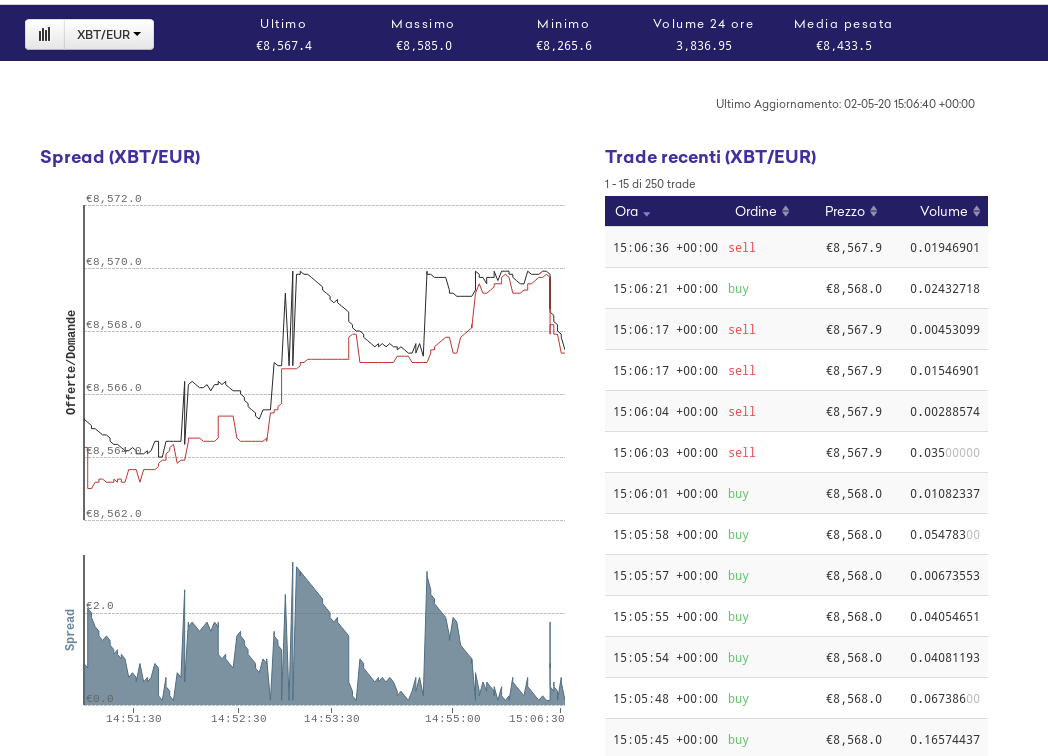
\includegraphics[width=10cm]{kraken_raw}
\end{center}
		\caption{\\~\\Figura: Elenco transazioni Bitcoin/Euro relative ad una finestra di minuti. I record mostrano l'ora in cui è avvenuto il trade, il tipo di operazione (buy / sell), il prezzo di scambio del titolo e la quantità di titoli scambiati. L'elenco dei dati di trade 'raw' è disponibile tramite le API kraken ed è la fonte grezza di dati finanziari utilizzati per calcolare i grafici OHLCV, fondamentali per l'analisi dei mercati. (fonte: https://www.kraken.com/)}
\end{fig}
\begin{fig}
\begin{center}
		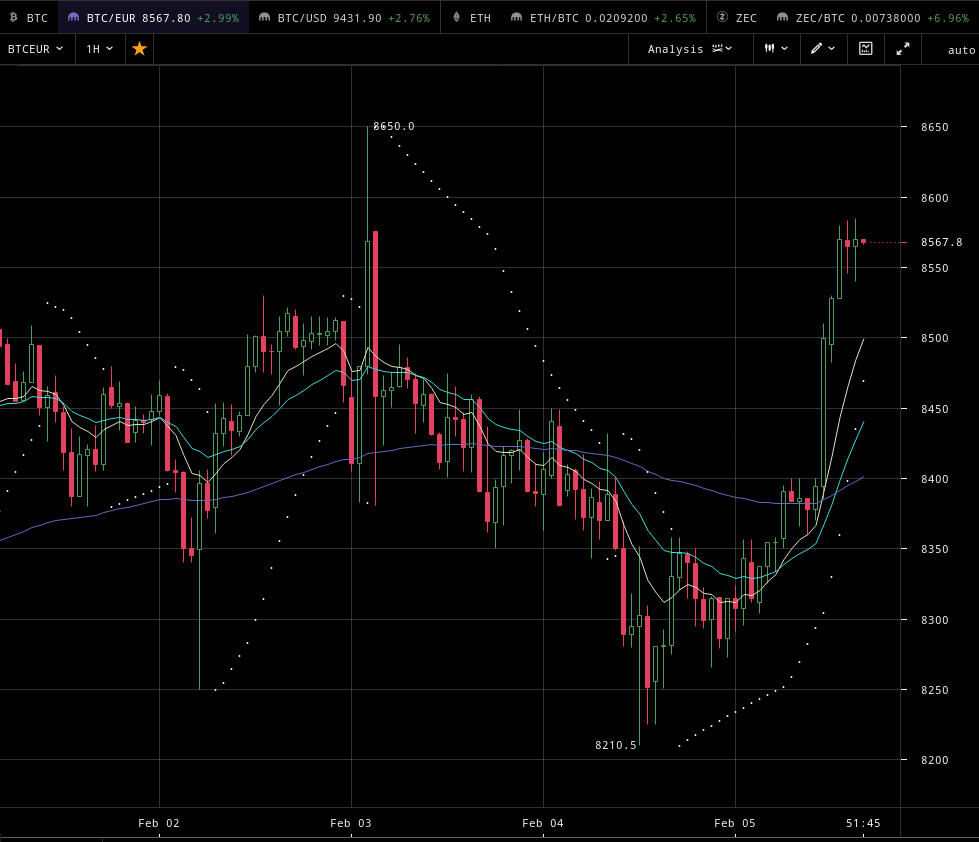
\includegraphics[width=\linewidth]{kraken_ohlcv}
\end{center}
		\caption{\\~\\Figura: Grafico OHLCV ricavato dai prezzi in Figura 1. Sulle ascisse è rappresentata l'ora mentre le ordinate sono il prezzo (in Euro) del titolo Bitcoin. Le "barre" orizzontali verdi e rosse sono le candele OHLCV: verdi se il prezzo è in crescita (\textit{open} minore di \textit{close}), rosse se in discesa (\textit{open} maggiore di \textit{close}). Le candele sono di durata 1 ora e quindi i prezzi elencati nella precedente immagine rientrano soltanto in parte nell'ultima candela (rossa) delle 15:00 - 16:00, ancora aperta e quindi in creazione. La candela è rossa perchè, come si nota dai prezzi, il valore del titolo  è in discesa: partendo da circa 8.568 (probabilmente più alto nei record precedenti) si scende verso 8.567.\\
			Le linee colorate rappresentano le medie mobili dei prezzi di chiusura; usate per analisi tecnica, sono rispettivamente le medie a 10 (verde), 21 (azzurro) e 100 (blu) candele. Più candele sono considerate nella media e meno questa cambierà bruscamente, avendo quindi la media a 100 candele (cioè 100 ore) molto più lenta delle altre. (fonte: https://www.kraken.com/)}
\end{fig}

Le immagini descrivono l'andamento dei prezzi scambio per scambio e le corrispondenti candele ohlcv come esposte dalla piattaforma di trading. I bordi orizzontali che compongono i lati superiore e inferiore della candela sono il prezzo di apertura e quello di chiusura: se la candela è rossa il prezzo di chiusura è minore di quello di apertura (significa che il prezzo dell'asset è sceso durante l'unità di tempo), e quindi il bordo superiore rappresenta il valore di \textit{open} e quello inferiore \textit{close}, mentre una candela verde indica una crescita del prezzo (\textit{open} è il lato inferiore mentre \textit{close} quello superiore). Le linee verticali della candela si estendono invece verso il prezzo minimo e massimo che l'asset ha toccato nel periodo di tempo fra apertura e chiusura della candela.
\\~\\
Le API di Kraken permettono di effettuare diversi tipi di operazioni, come scaricare lo storico dei prezzi di tutte le coppie valuta-criptovaluta disponibili, dal 2013; restare in attesa per ricevere in tempo reale i nuovi dati sugli scambi di titoli; inoltre è anche possibile creare il proprio portafogli sulla piattaforma e piazzare ordini di acquisto e vendita. Tutte funzionalità ben sfruttate da Sentyment, che opera sul mercato in autonomia.



\section{Gudagnare con il trading}
E' importante notare che la ricchezza in possesso, calcolata in ogni istante, è data dalla quantità di budget e dalla quantità di titoli posseduti. Gli asset finanziari hanno un valore monetario indicato dal loro prezzo, quindi il possesso di alcuni di questi, anche se il budget da investire è azzerato, comporta comunque una ricchezza investita che si può recuperare rivendendo il titolo.\\
Si prende come esempio l'asset XBT/EUR, valuta di scambio fra Bitcoin e Euro. Partendo da un budget iniziale in Euro, bisogna decidere quando comprare titoli di Bitcoin e quando rivenderli per avere di nuovo Euro. Lo scopo della AI, quindi, non è soltanto massimizzare gli Euro in possesso, ma anche il numero di titoli Bitcoin o del quantitativo di entrambi i titoli da avere in portafoglio che porti all'aumento del loro valore.\\
A seconda delle aspettative sul rialzo o ribasso di un titolo è possibile agire in due modi: andare \textit{long} o andare \textit{short}. Andare \textbf{long} vuol dire acquistare Bitcoin vendendo Euro, puntando ad un apprezzamento (aumento di valore) della criptovaluta; in questo caso l’aspettativa è di un aumento del valore del cambio e si avrà quindi una visione rialzista (bullish) del mercato. Andare \textbf{short} vuol dire vendere Bitcoin acquistando Euro, puntando quindi un apprezzamento dell'Euro nei confronti della criptomoneta. In questo caso l’aspettativa è di una diminuzione di valore del cambio. Si aprirà quindi una posizione che mira a una flessione del prezzo. La visione che il trader avrà del mercato sarà ribassista (bearish).\\~\\
Il punto centrale su cui si basano le strategie di investimento è indovinare se la valuta aumenterà o diminuirà di prezzo, per poi andare long o short a seconda della previsione. L'\textbf{analisi tecnica} è un metodo riconosciuto e largamente utilizzato per anticipare o prevedere l'andamento dei prezzi e si basa sull'aspetto tecnico del mercato, utilizzando grafici e dati storici. In particolare vengono analizzati prezzi, volumi scambiati e fasce temporali. Si utilizzano indicatori matematici, statistici e grafici e i segnali e i suggerimenti ricavati da questi strumenti accompagnano i trader nelle loro decisioni in merito all'apertura e chiusura di posizioni di trading. L'analisi tecnica è un metodo di previsione dei prezzi basato sui dati storici.
\\~\\
%		\textbf{Altro su analisi tecnica?
%		https://www.xtb.com/it/scuola-di-trading/che-cosa-e-lanalisi-tecnica}
Supponendo che il mercato ad un certo punto cresca e si abbia "indovinato" un buon numero di previsioni, ci si ritroverà a possedere dei titoli che ora valgono un prezzo superiore rispetto al loro valore iniziale. Se i titoli crescono di valore, è bene quindi acquistarne finchè salgono, in questo modo si possiede un maggior numero di asset che andranno a valere sempre di più; in caso di perdita di valore del titolo, invece, generalmente si dovrebbe vendere i titoli, per riacquistare del budget investito che ora stava perdendo valore e poterlo investire in altri titoli che crescono.\\
Quando si decide di acquistare si sta effettuando la seguente operazione: dato un certo budget iniziale \textit{budget}, il valore del titolo \textit{price} e la quantità di titolo acquistato \textit{equity} e supponendo di spendere sempre tutto il budget per acquistare il titolo
\\

\begin{equation}
equity=budget/price
\end{equation}
\\~\\
Mentre, all'occorrenza di un'operazione di vendita, utilizzando equity appena acquistata:\\

\begin{equation}
budget=equity*price
\end{equation}

\\~\\
È possibile in ogni momento calcolare il ricavo o quantità di beni in possesso combinando il budget con equity, tenendo presente che dopo un acquisto il budget scende a zero e equity assume il valore indicato, mentre dopo una vendita è equity a scendere a zero e si ritorna in possesso di budget. Lo stesso budget riacquistato verrà usato nuovamente per comprare dei titoli facendo così crescere di nuovo equity, e così via. Un vincolo è quello di non poter effettuare due medesime operazioni di fila. 
\\~\\
Se si considera un certo budget iniziale \textit{initial\_budget}, il \textbf{guadagno} (\textit{gain}) in ogni istante è dato da:
\\
\begin{equation}
gain=(budget+equity*price)-initial\_budget
\end{equation}

\\~\\
Questa è la formula del guadagno che verrà usata da qui in avanti.		
\\~\\\\~\\
A questo punto è necessario introdurre il concetto di \textbf{fee}.\\
Le varie piattaforme di trading addebitano un costo per ogni singola operazione, sia di acquisto che di vendita, intestandosi una percentuale di budget speso dai trader come tassa per mantenere la piattaforma stessa. Nel caso di operazioni di acquisto, la tassa è calcolata come percentuale del budget speso per comprare il titolo, quindi viene scalata subito e il risultato è l'acquisto di una quantità leggermente minore di titoli (la restante dei quali viene pagata alla piattaforma); per le vendite invece la fee è tolta dal budget una volta che questo è ricalcolato vendendo equity, risultando in un ricavo leggermente minore di quello che si sarebbe ottenuto vendendo realmente l'intera quantità di titoli.\\
Nel caso di Kraken, la piattaforma di trading di riferimento su cui opera Sentyment, le fee sono del 0.26\%: significa che viene sottratto il 0.26\% di budget che si intende investire, per ogni operazione. Per altri mercati, valute o piattaforme di trading le fee possono variare e potrebbero non essere basaste su una percentuale di acquisto ma fisse (flat fee vs per share fee).
\\~\\
La presenza delle fee modifica abbastanza drasticamente il funzionamento del mercato e l'efficacia delle strategie di investimento, che devono essere adattate ad un mercato con fee; è necessario quindi riscrivere le formule per il guadagno e per le operazioni di acquisto e vendita titoli, che ora comprendono la percentuale di fee.\\
Per gli acquisti, considerando un certo budget iniziale \textit{budget} (o il budget risultato di una precedente vendita), il valore del titolo \textit{price}, la quantità di titolo acquistato \textit{equity} e una tassa \textit{fee}:\\
\begin{equation}
equity=(budget*(1-fee))/price
\end{equation}
\\~\\
Per le vendite:\\
\begin{equation}
budget=(equity*price)*(1-fee)
\end{equation}
\\~\\
Dal momento che le budget e equity sono già calcolati togliendo le fee per ogni operazione di acquisto e vendita, la formula del guadagno rimane la stessa.\\~\\








%		\textbf{ESEMPIO DI COME CAMBIEREBBE RISULTATO CON E SENZA FEE CON POCHI DATI DI ESEMPIO?}










Senza addentrarsi nelle diversità dei titoli e dei mercati, si può affermare che una strategia generale e semplificata per guadagnare facendo trading è \textit{compra basso, vendi alto}; nella realtà i segnali di acquisto possono essere dati da altri indicatori più complessi e non sempre è possibile capire quando un titolo sta toccando un prezzo particolarmente alto o basso: è facile analizzare i grafici a posteriori, ma non altrettanto semplice prevedere massimi e minimi locali online. Per questo si utilizzano delle semplici strategie fondamentali che aiutano a capire l'andamento dei prezzi.


\section{Esempi di strategie}
Come già accennato, l'\textbf{analisi tecnica} è lo studio dell'andamento dei prezzi dei mercati finanziari nel tempo, allo scopo di prevederne le tendenze future, mediante principalmente metodi grafici e statistici. In senso lato è quella teoria di analisi secondo cui è possibile prevedere l'andamento futuro del prezzo di un bene quotato, studiando la sua storia passata. Viene utilizzata, assieme all'analisi fondamentale, per la definizione delle decisioni di operatività finanziaria.\\
L'analisi tecnica si prefigge di analizzare e comprendere, attraverso l'analisi del grafico, l'andamento dei prezzi, il quale a sua volta rispecchia le decisioni degli investitori; inoltre si basa sull'assunto fondamentale che, poiché il comportamento degli investitori si ripete nel tempo, al verificarsi di certe condizioni grafiche, anche i prezzi si muoveranno di conseguenza. Il compito principale dell'analisi tecnica è quindi quello dell'identificare un cambiamento di tendenza rispetto ad uno stadio iniziale, mantenendo una posizione di investimento fino a quando non vi sia prova che la tendenza stessa si sia di nuovo invertita.\\
Per individuare un trend si fa uso di indicatori tecnici, basati su prezzo e volume, calcolati a partire dai grafici: questi analizzano i movimenti di prezzo a breve termine e alcuni dei più noti e usati sono Moving Average Crossover, MACD (moving average convergence / divergence), RSI (relative strength index) e Bollinger Bands.\\
Analizzando i grafici passati mediante queste strategie è possibile ricavare i parametri per gli indicatori che meglio si adattano al mercato in analisi e riutilizzare l'indicatore, applicandolo ai dati futuri, per identificare nuovi trend.\\~\\

\subsection{Moving Average Crossover}
Questa strategia prevede il calcolo di una o più medie mobili a diverso periodo, le cui intersezioni nel grafico definiscono un segnale di buy o sell.\\
Il moving average crossover si verifica quando, nel grafico di due medie mobili ciascuna basata su diversi periodi, le linee di queste medie mobili si incrociano. Non prevede la direzione futura ma mostra le tendenze. Questo indicatore utilizza due (o più) medie mobili, una più lenta e una più veloce. La più veloce è una media mobile a breve termine. Per i mercati azionari di fine giornata, ad esempio, può essere un periodo di 5, 10 o 25 giorni mentre la più lenta è la media mobile di medio o lungo termine (ad esempio periodo di 50, 100 o 200 giorni). Una media a breve termine è più veloce perché considera i prezzi solo per un breve periodo di tempo ed è quindi più reattiva alle variazioni giornaliere dei prezzi. D'altra parte, una media mobile a lungo termine è considerata più lenta in quanto incapsula i prezzi per un periodo più lungo, tuttavia tende ad attenuare i disturbi che si riflettono spesso nelle medie mobili a breve termine.
\\
Una moving average, come una linea a sé stante, viene spesso sovrapposta nei grafici per indicare l'andamento dei prezzi. Un crossover si verifica quando una media mobile più veloce (cioè una media mobile di periodo più breve) attraversa una media mobile più lenta (cioè una media mobile di periodo più lungo).\\
In altre parole, accade quando la linea della media mobile del periodo più breve attraversa una linea della media mobile del periodo più lungo: questo punto di incontro viene utilizzato per comprare o vendere titoli (quando la media veloce supera quella lenta, si ha un segnale di \textit{buy}, mentre \textit{sell} se viceversa)
\\~\\
\begin{fig}
	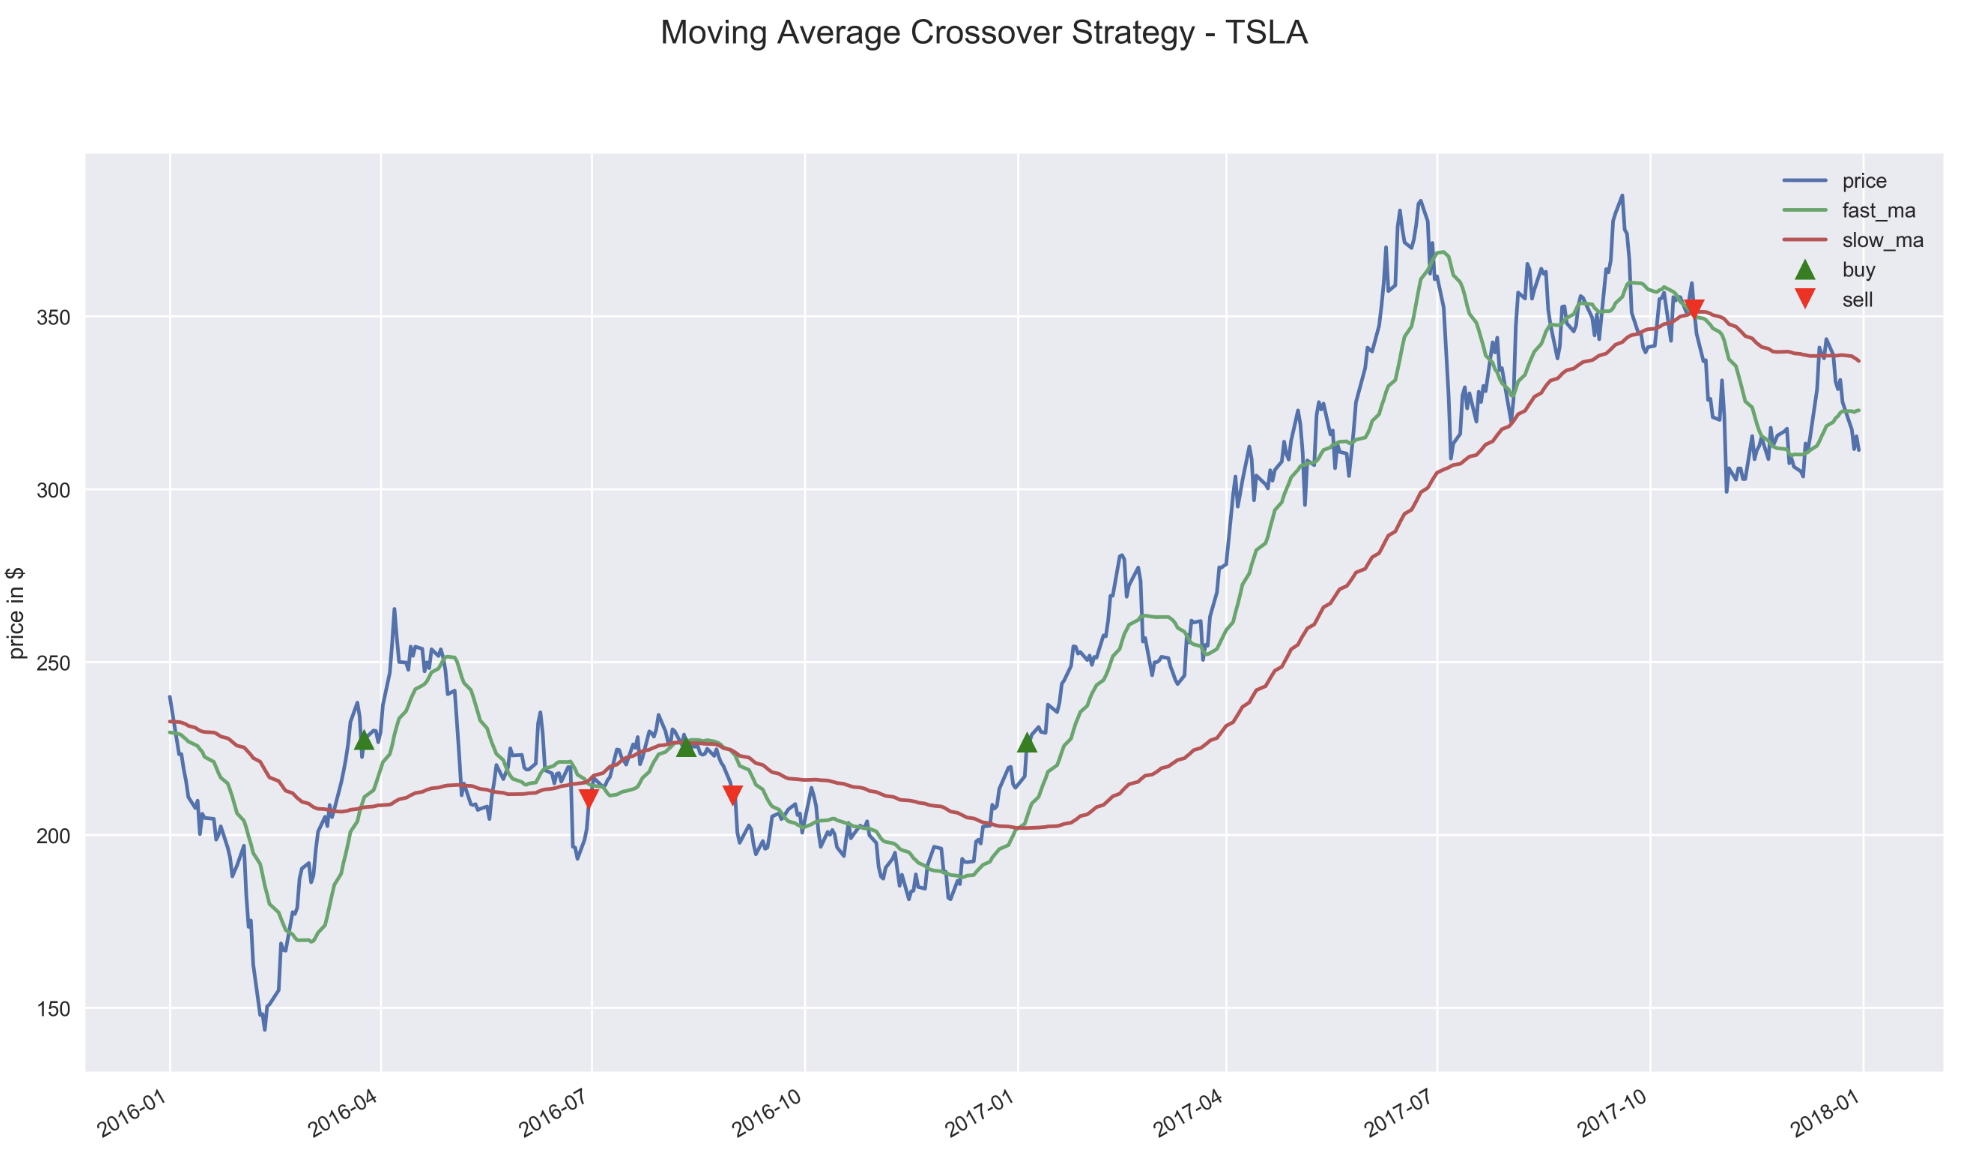
\includegraphics[width=\linewidth]{moving_avg}
	\caption{Figura: Andamento dei prezzi per il titolo TESLA/DOLLARO, accompagnato da due medie mobili a diverso periodo: fast\_ma a 20 giorni mentre slow\_ma a 100 giorni. Le frecce verdi e rosse indicano i segnali di buy e sell ricavati dalle intersezioni fra le medie}
\end{fig}

Ci sono diverse declinazioni della strategia a medie mobili, come ad esempio SMA (simple moving average), che utilizza come segnale di buy / sell il crossover fra i prezzi di chiusura e la media mobile semplice; EMA usa una media esponenziale; MACD (moving average convergence / divergence) usa come prima statistica la differenza fra la media veloce e quella lenta e, come seconda statistica, la media di queste differenze.
%		\\\textbf{PARLARE DI TUTTE LE STRATEGIE? MACD, RSI, BOLLINGER?}
\\~\\
Calcolati gli indicatori statistici più adatti alla situazione e scelti i parametri migliori (come i periodi delle medie da usare), si è costruito un modello di trend del titolo e si è in grado di prevedere quando il trend si ripropone. Prendendo l'esempio di una moving average crossover con una media veloce e una lenta, analizzato che per la maggior parte dei casi si riscontra un guadagno vendendo quando la media lenta supera quella veloce e comprando quando accade l'opposto, allora si può affermare che sarà molto probabile guadagnare ancora, in futuro, ripetendo le medesime operazioni.


\section{Ruolo delle intelligenze artificiali e scopo della tesi}		
L'apprendimento automatico e diverse tecniche hanno creato nuovi sistemi per individuare pattern, cosa che il cervello umano non è in grado di fare. Dal momento che la finanza è quantitativa, la AI nel trading azionario sta guadagnando terreno. Le società finanziarie hanno investito molto nell'intelligenza artificiale in passato e studiano e implementano le applicazioni finanziarie di machine learning e del deep learning nelle loro operazioni.\\
L'analisi tecnica è dunque implementata in sistemi automatici, che sono molto più efficienti di un trader umano e offrono diversi vantaggi. Le AI separano le informazioni prevedibili da qualsiasi "rumore casuale", gli algoritmi apprendono dall'accuratezza delle previsioni precedenti e si adeguano continuamente, abbastanza veloci da prevedere il mutamento della situazione del mercato anche in un orizzonte di pochi giorni. Possono imparare dai successi e fallimenti e riconfigurare ogni giorno le approssimazioni del funzionamento interno del mercato, poiché viene alimentato con nuovi dati.\\
Oltre agli indiscutibili vantaggi computazionali di una macchina rispetto al cervello, ci sono altri aspetti da considerare che hanno portato alla crescita delle AI nel settore. Si può infondere la conoscenza degli esperti dell'ambito in un software che si auto adatta e migliora, senza avere gli svantaggi dell'errore umano; si può estendere per permettergli di gestire diversi ambiti, dal recupero della materia prima (i dati di trading) fino alla vendita del prodotto finito (vendita di strategie di investimento). È possibile costruire sistemi complessi che modellano intere realtà.\\~\\
Sentyment è uno di questi software descritti. Si occupa di raccogliere dati, elaborarli e, attraverso una AI li analizza per produrre strategie di investimento. Il modulo di intelligenza artificiale è molto ampio: esistono molte AI che operano producendo costantemente nuovi segnali di buy / sell per le strategie e sono monitorate da una ulteriore, singola AI. Questo supervisore decide quale fra le molte AI sta avendo più successo e la promuove come attiva da utilizzare.\\
Lo scopo della tesi è sviluppare il supervisore e inserirlo all'interno del complesso sistema di Sentyment, impiegando tecniche di test per intelligenze artificiali che permettano di scegliere un rappresentante migliore fra una serie di agenti che operano indipendentemente.


\newpage
\chapter{Sentyment}
\label{cap2}

Sentyment è il prodotto di un'azienda milanese che opera nel settore informatico-finanziario. Nexid Edge è un ramo del gruppo NEXiD votato per perseguire l'innovazione tecnologica e sviluppare soluzioni di digital business rivoluzionarie. SentYment è la nuova Business Unit dedicata all'intelligenza artificiale.\\
L'obiettivo è offrire alle organizzazioni un accesso senza pari a tecnologie all'avanguardia che uniscono il meglio della tecnologia e dell'imprenditorialità per elevare la saggezza collettiva. Al momento, grazie all'intensa collaborazione con Nexid Finance, Nexid Edge è attiva nel fornire progetti di consulenza digitale end-to-end, per offrire ai clienti un'esperienza di \textit{augmented consulting}. \footnote{Nexid, Srl. URL: https://nexid.it/}\\
In questo documento, tuttavia, si fa riferimento a "Sentyment" intendendo l'applicazione sviluppata e non la divisione AI di Nexid.
\\~\\

Essendo il fine ultimo della tesi l'inserimento un nuovo modulo operativo in Sentyment, è necessario prendere familiarità con il software e i dati che tratta.\\
L'applicazione di intelligenza artificiale era già esistente e in grado di raccogliere dati da Kraken e produrre le strategie ma mancava di un'architettura modulare, di componenti separati che assolvono a ruoli precisi e definiti e di un'interfaccia ad API per interrogare il sistema in esecuzione. Era quindi necessario sviluppare da zero \textit{data module} e \textit{coordinator} e permettere l'integrazione del resto del sistema già esistente nella nuova architettura a moduli. Era inoltre richiesto lo sviluppo della nuova AI di controllo, supervisore che sceglie la migliore fra le AI in esecuzione.\\
Tutti i moduli del sistema sono scritti in Python3, comprese le AI stesse. Alcune loro parti sono state riscritte in Cython e Go per migliorare le prestazioni.

\begin{fig}
	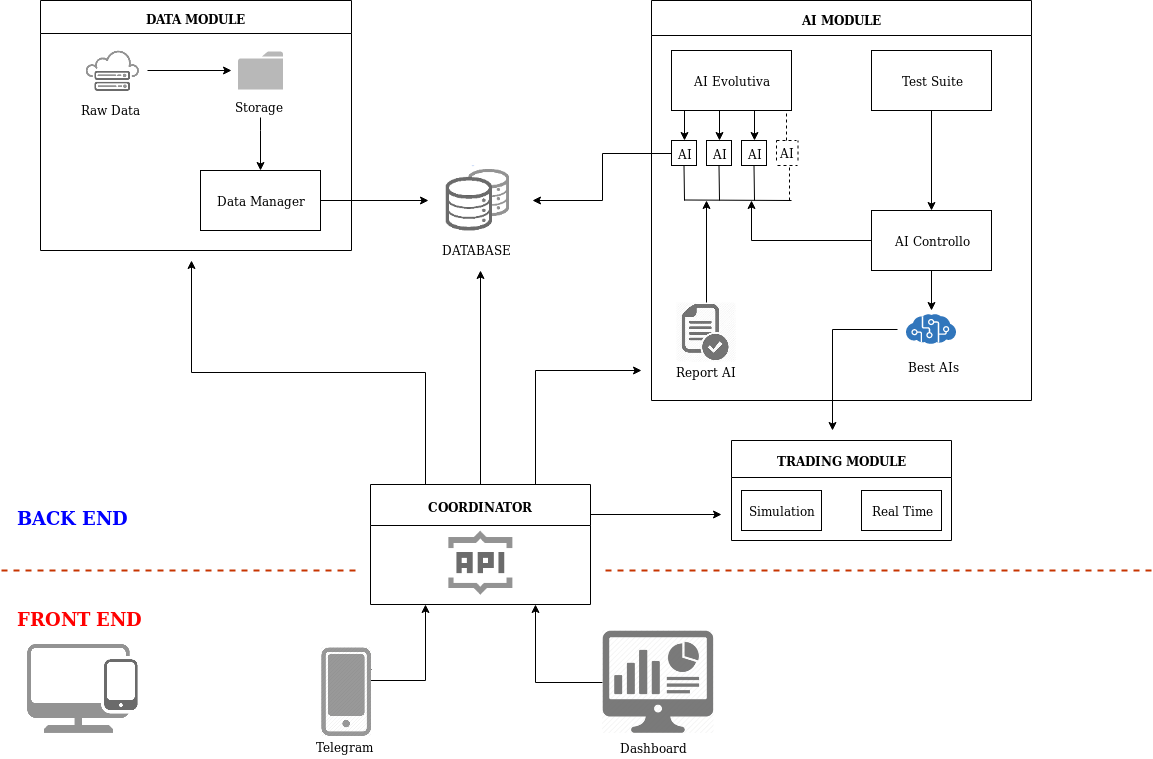
\includegraphics[width=\linewidth]{Sentyment}
	\caption{\\~\\Figura: Architettura di Sentyment. Nei riquadri sono mostrati i quattro principali componenti, suddivisi al loro interno in ulteriori sotto-moduli. Il grafico è diviso in \textit{front-end} e \textit{back-end}, che rappresentano rispettivamente le interfacce esposte all'utente utilizzatore del sistema, e la parte di logica non accessibile dall'esterno}
\end{fig}
\\~\\

Verranno ora brevemente presentati i componenti di Sentyment.
\begin{itemize}
	\item \textit{data module} raccoglie i record di trade raw tramite le API Kraken, gestisce la creazione e scrittura delle candele OHLCV e permettere l'accesso a tutti i dati e i database da parte degli altri componenti. I sotto-moduli si spartiscono i compiti: quando i dati di trade sono scaricati e salvati su uno storage temporaneo da \textit{raw data}, allora \textit{data manager} li copia sul database permanente e in automatico scatta la creazione delle nuove candele OHLCV, che sono create allo scoccare della nuova ora a partire dai dati appena scaricati (o minuto/giorno, a seconda delle configurazioni scelte). Infine le nuove candele create sono inserite nel database.
	\item \textit{coordinator} implementa le interfacce esposte per il controllo e l'interrogazione dello stato di Sentyment. È l'unico punto di accesso al sistema in esecuzione. Tramite delle API esposte su server è possibile conoscere quali asset sono attualmente in fase di scaricamento e le informazioni riguardo le configurazioni delle candele che si vogliono creare; è inoltre possibile impostare i timeframe delle candele (orarie, giornaliere), attivare o disattivare i download dati e forzare la creazione di specifiche candele.
	\item \textit{AI module} è la parte preesistente di intelligenza artificiale. Contiene le numerose AI che creano le strategie di investimento e il supervisore che sceglie la migliore fra queste, a intervalli fissati. È inoltre presente un modulo che crea report che descrivono l'andamento delle AI, i dati che stanno processando e le statistiche calcolate per ognuna di esse, per misurarne la performance online.
	\item \textit{trading module} si occupa di seguire le strategie create dalle AI per effettuare direttamente operazioni di acquisto e vendita tramite le API di Kraken. È collegato ad un portafoglio Kraken che contiene un certo budget ed è libero di fare trading. Oltre ad agire sul mercato vero, le AI operano anche in un ambiente simulato che permette di riprodurre e monitorare quale sarebbe stato il loro comportamento nel mercato reale o in nuovi mercati non ancora raggiunti, al fine di calcolare ulteriori statistiche e tracciare l'evoluzione delle AI.
\end{itemize}

Come già accennato, sono stati sviluppati \textit{data module} e \textit{coordinator}, ridisegnando la preesistente architettura di Sentyment e integrando gli altri componenti. Durante la riprogettazione si sono potute scegliere liberamente la logica di implementazione e le tecnologie da impiegare, con la restrizione di dover utilizzare Python3, con \textit{sqlalchemy}\footnote{SQLAlchemy è un toolkit SQL open-source e object-relational mapper (ORM) per Python} come \textit{ORM}\footnote{l'Object-Relational Mapping (ORM) è una tecnica di programmazione che favorisce l'integrazione di sistemi software aderenti al paradigma della programmazione orientata agli oggetti con sistemi RDBMS (Relational Database Management System). Un prodotto ORM fornisce, mediante un'interfaccia orientata agli oggetti, tutti i servizi inerenti alla persistenza dei dati, astraendo nel contempo le caratteristiche implementative dello specifico RDBMS utilizzato.} e \textit{flask}\footnote{Flask è un micro framework web scritto in Python. Ha un nucleo semplice ma estendibile: ci sono ad esempio estensioni per la validazione delle form, la gestione del caricamento dei file, varie tecnologie di autenticazione ed altro} per implementare il server e le API.\\
Prima di sviluppare la AI supervisore sono state testate le AI singolarmente attraverso alcune metodologie di test che saranno descritte di seguito. È stato svolto un lavoro di analisi dei dati prodotti dalle AI, confrontandoli con alcune strategie di base e con altre intelligenze artificiali sviluppate al fine di misurarne le prestazioni e solo dopo le AI sono state confrontate fra di loro. I metodi ritenuti migliori per il confronto sono stati scelti in seguito ad un'analisi del contesto e alla natura finanziaria dei dati.

\section{Strumenti e tecnologie utilizzati}
Sentyment è quasi totalmente scritta in Python3, tranne per alcune parti in cui si ha bisogno di elevate performance che sono quindi state riscritte in Cython\footnote{Cython è un linguaggio di programmazione che mira ad essere un superset del linguaggio di programmazione Python, progettato per fornire prestazioni di tipo C con codice scritto principalmente in Python con sintassi aggiuntiva opzionale ispirata al C}. Queste comprendono, ad esempio, gran parte del codice delle AI, ma non solo.\\
Si fa uso estensivo di librerie di analisi dati quali \textit{numpy}\footnote{NumPy è una libreria open source per il linguaggio di programmazione Python, che aggiunge supporto a grandi matrici e array multidimensionali insieme a una vasta collezione di funzioni matematiche di alto livello per poter operare efficientemente su queste strutture dati.}, \textit{pandas}\footnote{Pandas è una libreria software scritta per il linguaggio di programmazione Python per la manipolazione e l'analisi dei dati. In particolare, offre strutture dati e operazioni per manipolare tabelle numeriche e serie temporali. Il nome deriva dal termine "panel data", termine econometrico per set di dati che include osservazioni su più periodi di tempo per gli stessi individui.} e \textit{matplotlib}\footnote{Matplotlib è una libreria per la creazione di grafici per il linguaggio di programmazione Python e la libreria matematica NumPy. Fornisce API orientate agli oggetti che permettono di inserire grafici all'interno di applicativi} per visualizzare i grafici dei dati, soprattutto nella parte di sviluppo e analisi.\\
Queste librerie sono i classici strumenti utilizzati nell'analisi dati con Python e sono i più utilizzati; le alternative attualmente presenti non offrono le stesse funzionalità con la medesima efficienza e per questo erano anche i \textit{tool} già usati nella prima versione di Sentyment.\\
Pandas, in particolare, permette di importare grandi quantità di dati direttamente da database o da file ed è in grado di gestirli in modo efficiente indicizzandoli e garantendo un accesso rapido. Un ampio set di operazioni statistiche sui dati lo rende uno strumento indispensabile in \textit{data science} e ampiamente utilizzato. Basti pensare ad un AI a cui servono in input moltissimi dati: quando questi sono salvati su database è facile eseguire piccole letture e query puntuali e aggregate ma quando, invece, si ha bisogno di portarne in memoria un gran numero per processarli con funzioni al di là delle potenzialità di \textit{SQL}, serve un ulteriore strumento capace di gestire l'accesso efficiente alla memoria e che offra direttamente queste funzioni di analisi (esempio con funzione \textit{resample} nel Capitolo 3).\\~\\

Il database scelto è di tipo \textit{relazionale}. Si è scelta l'opzione relazionale invece di \textit{noSQL} in quanto i dati sono tutti perfettamente strutturati (schema dati in dettaglio nel Capitolo 3): la sorgente principale da cui partono tutte le elaborazioni è rappresentata dai dati di trading \textit{raw} forniti da Kraken. Questi hanno ciascuno un riferimento al \textit{timestamp}, alla tipologia dell'operazione di trade, la quantità di titoli venduti / acquistati e il loro volume. Sostanzialmente non servono altre informazioni per la creazione delle candele OHLCV, che sono anch'esse strutturate ed esplicitano \textit{open}, \textit{high}, \textit{low}, \textit{close}, \textit{volume}, \textit{timestamp} finale e altri dati secondari. Le AI lavorano tutte sulle candele e necessitano soltanto degli attributi appena citati.\\~\\
L'unica eccezione, in cui dati non sono perfettamente strutturati, sono le AI. Sono memorizzate come un insieme di parametri che permettono la loro ricreazione in un secondo momento, se necessaria, e sono salvati in formato \textit{JSON}.\footnote{JSON, acronimo di JavaScript Object Notation, è un formato adatto all'interscambio di dati fra applicazioni client/server. È basato sul linguaggio JavaScript ma ne è indipendente.} Dato che i parametri sono diversi, non strutturati e con possibilità di molteplici valori nulli, la memorizzazione in JSON già adottata nella prima versione di Sentyment sembrava comunque adatta, permettendo una compressione più efficiente dei dati e un accesso orientato al documento. Di una specifica AI si vogliono conoscere i suoi parametri, ma il nome / \textit{id} della AI é noto: per esempio, in seguito ad un'analisi durante un nuovo ciclo di test / sviluppo, si vuole continuare dalla AI più promettente fra quelle della precedente iterazione e quindi si accede al documento che contiene tutti i parametri della AI scelta.\\
I JSON dei parametri delle AI non sono scritti su database, ma sono dei file che risiedono direttamente su file system nelle directory di Sentyment, strutturate in modo da poter accedere ai parametri di una certa AI usando il suo identificativo. In sviluppi futuri potrebbe essere più adatto l'uso di un database non relazionale per la memorizzazione delle AI, oppure sfruttare i tipi di dato JSON presenti in ormai tutti i RDMBS moderni e quindi salvare tutto nello stesso database.\\~\\
Fra i database relazionali è stato scelto \textit{Mysql}\footnote{MySQL o Oracle MySQL è un Relational database management system (RDBMS) composto da un client a riga di comando e un server. È un software libero rilasciato a doppia licenza ed è sviluppato per essere il più possibile conforme agli standard ANSI SQL e ODBC SQL. I sistemi e i linguaggi di programmazione che supportano MySQL sono molto numerosi.} perché meglio si sposa con l'ORM di \textit{sqlalchemy}.\\~\\

Sqlalchemy permette di manipolare database SQL direttamente da Python. Mappa lo schema tabellare dei dati in uno a oggetti più facilmente processabile dal linguaggio di programmazione scelto, in questo caso Python. Grazie alla tecnologia degli ORM, il modello dei dati è sempre disponibile come classe del linguaggio e risulta quindi più comodo il loro accesso e manipolazione: ora si lavora con collezioni di oggetti invece che con un semplice elenco di record contenenti alcuni campi.\\
L'ORM mette anche a disposizione un motore di astrazione per le \textit{query}. Tramite un modello ad API le query eseguite in Python sono tradotte nel dialetto SQL del DBMS sottostante. Al programmatore resta il compito di scrivere le query usando l'\textit{expression language}\footnote{Expression Language (EL) è un linguaggio per creare una rappresentazione interpretabile di conoscenze specifiche. In questo caso è un linguaggio creato da sqlalchemy appositamente per rappresentare query SQL nel linguaggio di Python.} di sqlalchemy, il sistema usato per rappresentare strutture dei database relazionali e espressioni usando Python.\\~\\

\textit{Flask}, infine, è un microframework per Python ed implementa \textit{coordinator}, il web server che espone le informazioni disponibili sullo stato di esecuzione di Sentyment. È molto minimalista se mantenute le impostazioni di default e serve soltanto documenti JSON e non pagine HTML.\\
In futuri sviluppi le informazioni fornite dal web server in JSON potrebbero essere processate da un ulteriore componente, che le esporrebbe in modo più user-friendly attraverso un software di front-end e permetterebbe l'interrogazione di \textit{coordinator}, attraverso le API, in maniera più intuitiva.


\newpage
\chapter{Criptovalute}
Intro bitcoin? perche' sentyment si focalizza su queste e 2 parole di intro su come fare trade rispetto a valute normali?
Ethereum ha tante cose interessanti tipo smart contract e linguaggio solidity.

\newpage
\chapter{Elaborazione dati di trading}
\label{cap3}
In questo capitolo si andrà principalmente a descrivere il lavoro svolto dal software di raccolta e gestione dati, \textit{data module}, e alcuni dettagli della sua implementazione. Attraverso l'analisi delle operazioni svolte dal programma si darà anche un ulteriore sguardo ai dati, a come sono organizzati dalla piattaforma di trading e all'interno del software di Nexid, e a come si processano per ottenere un formato utile per l'elaborazione da parte delle AI.\\
Anche se Sentyment comprendeva già una parte di logica di scaricamento dati, in seguito alla sua riorganizzazione è stato necessario riscrivere questa parte di software convertendola interamente in un modulo separato, sempre attivo e pronto a scaricare, con cui si può interagire attraverso \textit{coordinator}. Svolge diverse attività fra cui scaricare grazie alle API di Kraken, creare le candele OHLCV a partire dai dati scaricati e gestire il database.\\~\\
I requisiti dell'applicativo sono i seguenti:
\begin{itemize}
	\item Scaricare dati di trade \textit{raw} per diversi tipi di asset, restando aggiornati in tempo reale con l'arrivo di nuovi
	\item Fornire la possibilità di scaricare dati passati
	\item Creare candele OHLCV a partire dai dati scaricati e poter sceglierne i parametri (lunghezza candela, periodo da considerare)
\end{itemize}

\section{Download dati Kraken}
L'input di tutto il sistema sono i dati di trade. Un modulo intero è dedicato alla logica di scaricamento dati, il cui fine è soltanto fornire i suddetti dati alle intelligenze artificiali, che rappresentano la parte principale del software. Tutta l'architettura è orientata al dato; le AI stesse ignorano l'esistenza di \textit{data module}, perché di fatto accedono direttamente al database per prelevare i dati, ignorando chi lo abbia riempito. Un metodo strutturato per "riempire" il database e preparare i dati per le AI è quindi un passo iniziale e fondamentale per tutta l'architettura.\\~\\
Le API di Kraken si dividono in \textit{pubbliche} e \textit{private}: tutte le attività svolte da \textit{data module} fanno uso soltanto delle interfacce pubbliche, mentre quelle private, le quali necessitano di un API Key\footnote{Una chiave per API (API Key) è un identificatore univoco utilizzato per autenticare un utente, uno sviluppatore o il programma chiamante un'API. Tuttavia, vengono in genere utilizzati per autenticare un progetto con l'API anziché un utente umano. Spesso si usano per accedere a quelle API che forniscono servizi a pagamento o per superare limitazioni di utilizzo.}, servono per collegare un portafoglio con budget e permettono di eseguire operazioni di acquisto e vendita di titoli. Sono utilizzate soprattutto dal modulo di trading.\\
Le API pubbliche permettono molti tipi di operazioni fra cui, le più usate:
\begin{itemize}
	\item \textbf{Get tradable asset pairs}: elenco di tutti gli asset trattati da Kraken,i \textit{ticker}\footnote{Il ticker è un’abbreviazione che identifica le società che vengono quotate su un mercato finanziario. Quando una società decide di ‘diventare pubblica’, sceglie il tipo di mercato sui cui essere quotata e il ticker di identificazione. Il ticker viene chiamato anche ticker azionario oppure ticker simbolo. Il termine deriva in effetti dal ‘ticker tape’ o ‘nastro per telescrivente’, un nastro su cui, nel passato, si trasmettevano le informazioni relative ai prezzi.}, con associato il nome usato e altre informazioni. Sono 110 in totale le coppie di valute di scambio fra una criptovaluta e la sua controparte in Euro o Dollaro. Alcuni esempi:
	\begin{itemize}
		\item XXBTZEUR: ticker che rappresenta la valuta Bitcoin-Euro (XBT-EUR)
		\item XXBTZUSD: Bitcoin-Dollaro (XBT-USD)
		\item XETHZEUR: Ethereum-Euro (ETH-EUR)
		\item XETHZUSD: Ethereum-Dollaro (ETH-USD)\\
		
		Non ci sono soltanto valute di scambio fra Euro / Dollaro e una criptovaluta, ma bensì anche scambi fra criptovaluta e criptovaluta, come, ad esempio:
		\item ADAETH: valuta di scambio fra le due criptovalute Cardano (ADA)\footnote{Cardano è una piattaforma che gestisce la criptovaluta ADA. Il progetto è guidato dall'ex co-fondatore di Ethereum. Lo scopo di Cardano è creare una piattaforma adatta allo sviluppo di smart contracts e un sistema di pagamento (altro sulle criptovalute nel Capitolo 3).} ed Ethereum (ETH)
		\item XZECXXBT: Zcash (ZEC)\footnote{Zcash è una criptovaluta che offre privacy e trasparenza selettiva delle transazioni. I pagamenti Zcash sono pubblicati su una blockchain pubblica, ma il mittente, il ricevente e il valore della transazione possono rimanere privati. Come Bitcoin Zcash ha una fornitura fissa totale di 21 milioni di unità.} e Bitcoin (XBT)\\
		
		Gli asset che scambiano due criptovalute fanno parte dei ticker gestiti da Kraken e quindi sono comunque scaricati e memorizzati nel database, ma non verranno usati nel resto del progetto.
		
	\end{itemize}
	
	L'elenco è scaricato in una fase iniziale di setup del modulo dati e ha lo scopo di memorizzare su database i nomi usati da Kraken per tutti gli asset che fornisce, in modo da poterli utilizzare nelle altre API per la fase successiva, in cui si richiede l'elenco di trade di uno specifico ticker.\\Come si può notare sono usati nomi particolari per rappresentare i ticker ed è quindi necessario memorizzare il mapping fra nome reale e nome usato da Kraken per poi poter utilizzare le API che seguono.\\
	%TODO: Esempio JSON ritornato?
	
	\item \textbf{Get recent trades}: Ora che si conoscono i nomi dei ticker usati da Kraken si possono usare per richiedere, per ciascuno di essi, l'elenco delle transazioni di mercato. Questa è in assoluto la API più usata dal modulo dati: riceve i dati di trade \textit{raw} che costituiscono l'input principale da cui partono le successive elaborazioni. I dati di trade sono memorizzati e saranno usati per creare le candele OHLCV, l'input per le intelligenze artificiali.\\
	Attraverso questa API è possibile sia richiedere dei dati storici in un certo periodo di tempo passato, sia ricevere aggiornamenti sui nuovi dati disponibili. In entrambi i casi va specificato come parametro il ticker di cui si vuole conoscere l'elenco degli scambi. Come secondo parametro è necessario un riferimento temporale che indichi quali trade sono richiesti di preciso (parametro \textit{since}).\\~\\%TODO: riferimento a BUCHI KRAKEN? da mettere tipo alla fine fine???
	Esempio di documento JSON restituito dalla chiamata a questa interfaccia, usando come parametri il ticker XXBTZEUR e il riferimento a gennaio 2020:
	\begin{verbatim}
	{
	  "error":[],
	  "result":
	  {
	    "XXBTZEUR":
	    [
        ["6410.20000","0.07588465",1577833204.9008,"b","m",""],
        ["6410.00000","0.02911527",1577833220.5154,"s","l",""],
        ["6410.00000","0.02910911",1577833261.2323,"s","l",""],
        ["6435.50000","0.08000000",1577842069.8177,"s","l",""], ...
	    ]
	    "last":"1577842069817694680"
	  }
	}
	\end{verbatim}

	Otre ad alcuni metadati utili per riutilizzare le API, sono principalmente elencati una serie molto lunga di record formati da sei campi: \textit{price}, \textit{volume}, \textit{time}, \textit{buy/sell}, \textit{market/limit}, \textit{miscellaneous}.\\ Prendendo come esempio il primo record:
	\begin{itemize}
		\item \textit{price}: 6410.20000. Siccome la valuta è Bitcoin-Euro, il numero indica il valore di un titolo Bitcoin espresso in Euro.
		\item \textit{volume}: 0.07588465. La quantità di titoli Bitcoin scambiati in quell'istante.
		\item \textit{time}: 1577833204.9008. Timestamp associato all'operazione in formato unix timestamp.\footnote{Nei sistemi operativi Unix e Unix-like il tempo viene rappresentato come offset in secondi rispetto alla mezzanotte del 1º gennaio 1970. I decimali rappresentano la frazione di secondo.}
		\item \textit{buy/sell}: "b". Indicazione del tipo di operazione: 'b' (buy) o 's' (sell).
		\item \textit{market/limit}: "m". Indica se comprare a prezzo di mercato (m) o se applicare un limit. Un limit order è un ordine inserito nell’order book con un prezzo limite specifico. Quando è inserito un limit order, l’operazione verrà eseguita solo se il prezzo di mercato raggiunge il prezzo limite. È quindi possibile usare limit order per comprare a un prezzo più basso o per vendere a un prezzo più alto rispetto all’attuale prezzo di mercato.
		\item \textit{miscellaneous}: "". Spazio per eventuali commenti o casi particolari.
	\end{itemize}
	
	
	Il campo \textit{last} serve da passare come nuovo parametro \textit{since} nella prossima chiamata, a indicare di scaricare ancora i dati dal punto in cui ci si era fermati. Siccome il volume dei dati di trade è molto elevato,\footnote{I dati di trade di Bitcoin per il solo anno 2019 hanno un'occupazione dell'ordine di grandezza dei 10 Gb.} viene diviso in frammenti; per continuare a scaricare frammento per frammento si sfrutta la combinazione di questi due parametri.
	
	\item \textbf{Get OHLC data}: Kraken offre anche la possibilità di scaricare direttamente le candele OHLCV create a partire dai dati di trade raw, ma questa funzionalità è già implementata all'interno di Sentyment stesso. Ad ogni modo, sono comunque riportati alcuni esempi di dati scaricati tramite questa API.\\
	Esempio di documento JSON restituito dalla chiamata, con parametri il ticker XXBTZEUR, il timestamp di gennaio 2020 e la lunghezza di candela a un minuto:
	\begin{verbatim}
	{
	  "error":[],
	  "result":
	  {
	    "XXBTZEUR":
	    [
	      [1582093500,"9384.7","9384.7","9384.6","9384.6","9384.6",
	        "0.35398923",9],
	      [1582093560,"9384.6","9384.7","9384.0","9384.0","9384.5",
	        "0.04147968",5],
	      [1582093620,"9384.1","9384.1","9384.0","9384.0","9384.0",
	        "0.40413908",5],
	      [1582136640,"9433.6","9433.6","9433.5","9433.5","9433.5",
	        "0.33265963",4], ...
	    ],
	    "last":1582136580
	  }
	} 
	\end{verbatim}
	
	La struttura del documento è simile a quella restituita nell'esempio precedente, con la differenza che ora i record sono composti da attributi diversi. Prendendo come esempio il primo record:
	\begin{itemize}
		\item \textit{time}: 1582093500. Timestamp finale della candela. La candela delle 12:00 comprende i trade dalle 11:00 alle 11:59.
		\item \textit{open, high, low, close}: rispettivamente 9384.7, 9384.7, 9384.6, 9384.6. Prezzo di apertura e chiusura della candela, minimo e massimo.
		\item \textit{vwap}: 9384.6. Prezzo medio della candela.\footnote{In finanza, Volume Weighted Average Price (VWAP) è il rapporto tra il valore scambiato e il volume totale scambiato in un determinato orizzonte temporale. È una misura del prezzo medio al quale un titolo viene negoziato nell'orizzonte di negoziazione.}
		\item \textit{volume}: 0.35398923. Somma totale della quantità di titoli scambiati durante l'intervallo di tempo della candela.
		\item \textit{count}: 9. Numero di operazioni buy / sell realmente eseguite all'interno della durata della candela.
	\end{itemize}

	Il significato e la definizione degli attributi delle candele verranno trattati in dettaglio più avanti.\\
	Il modulo di scaricamento è molto semplice e interroga solamente le API di Kraken, memorizzando di volta in volta blocchi di dati su database. L'unica difficoltà incontrata risulta essere la comprensione di alcuni parametri delle API, che si dimostrano non perfettamente documentate e pertanto è lasciato ai programmatori scoprire il significato di alcune interfacce.\\
	Per esempio il parametro \textit{last}, che dovrebbe indicare l'ultimo timestamp fra i record ritornati nella chiamata e che va passato come parametro \textit{since} nella successiva chiamata, per ripartire dall'ultimo trade, è controverso. La documentazione riporta "\textit{return trade data since given id}", intendendo quindi che si tratti di un identificatore: curiosamente in moltissimi casi (soprattutto nei dati OHLC, che hanno tutti timestamp preciso all'ora) ha lo stesso valore del timestamp e quindi questo significa che i timestamp sono usati come id. Quando, però, il valore ha dei decimali, che nel caso di un unix timestamp indicano frazioni di secondo, questi sono aggiunti in coda all'identificatore con un \textit{padding}\footnote{Il padding è una delle numerose pratiche che prevedono l'aggiunta di dati all'inizio, a metà o alla fine di un messaggio. È usato per rendere uniforme un certo dato, allineandolo alla lunghezza specificata: se la lunghezza del messaggio finale deve assumere precisamente un certo valore ma il testo contenuto è più breve, si aggiungono tanti valori di padding quanti la differenza fra la lunghezza del messaggio da inviare e quella del testo contenuto.} a 0 di nove cifre. Quando si richiedono i dati a partire da un certo timestamp che non ha decimali, quindi, bisogna aggiungere il padding altrimenti l'id richiesto non viene trovato nei database di Kraken. In risposta è invece ritornano il record con id minore di tutti, che è quello che più si avvicina al valore richiesto, estremamente basso rispetto a tutti gli altri id presenti nel database dato che ha nove cifre mancanti.\\~\\
	Tutte queste informazioni si possono inferire analizzando molte chiamate con argomenti particolari ma non vi è una documentazione completa che espone chiaramente l'uso corretto del parametro e il risultato sono dei comportamenti inaspettati nei programmi che usano le API. Una volta capito il problema è facile aggirarlo, ma la scelta progettuale di utilizzare i timestamp convertiti a id è discutibile e inoltre non chiaramente documentata.

	
\end{itemize}

\section{Creazione candele OHLCV}
%TODO: Formule di ohlcv e esempi con immagini e tabelle di creazione
Una volta memorizzati tutti i dati di trade raw e disponibili per le letture, è il momento di creare il dato aggregato che riassume le operazioni di scambio e che rappresenta la principale fonte di input per le intelligenze artificiali.\\~\\
Le candele sono interamente generate grazie alla libreria di Python \textit{pandas}, chiamando il metodo \textit{resample}\footnote{Da documentazione pandas: https://pandas.pydata.org/pandas-docs/stable/reference/api/pandas.DataFrame.resample.html}:
\begin{verbatim}
def resample(self, rule, ... ):
	Resample time-series data.
	
	Convenience method for frequency conversion and resampling of time series.
	Object must have a datetime-like index (DatetimeIndex, PeriodIndex, 
	or TimedeltaIndex), or pass datetime-like values to the on or level keyword.
	
\end{verbatim}

È un metodo della classe DataFrame, quindi viene chiamato a partire da un oggetto contenente il dataset da ricampionare per creare la candela; come parametro è usato \textit{rule}, un \textit{timedelta} che rappresenta la lunghezza della candela.
\\~\\
Supponendo di avere dunque tutti i dati raw disponibili nel database e di voler creare candele con timeframe di un'ora, per tutto il mese di gennaio 2020, il procedimento seguito è il seguente:

%TODO pseudo algo leggi db - resample - scrivi su db

\\~\\
Dal punto di vista concettuale, il metodo citato aggrega i dati creando un nuovo record contenente i quattro attributi \textit{open}, \textit{high}, \textit{low}, \textit{close}, \textit{volume}. Formalmente:
\begin{itemize}
	\item \textit{open}
	\item \textit{high}
	\item \textit{low}
	\item \textit{close}
	\item \textit{volume}: sommatoria singoli volumi %TODO: formula 
\end{itemize}

Dove, per ogni record, \textit{price} è il prezzo dell'asset scambiato, \textit{volume} è....


%TODO: un esempio numerico di dati raw e risultato resample

\section{Indicatori}
%TODO: Formule e esempi calcolo indicatori SMA EMA MACD RSI e altre statistiche

\section{Creazione strategie}

\newpage
\chapter{Test per intelligenze artificiali}	
\label{cap4}
% https://www.forbes.com/sites/cognitiveworld/2020/01/03/how-do-you-test-ai-systems/#48ba5d76afd5

I test sono in realtà un elemento chiave per il funzionamento dei progetti di intelligenza artificiale. Non si sviluppa semplicemente un algoritmo AI fornendo dati di training e mettendolo in produzione; è necessario verificare effettivamente che i dati di addestramento svolgano un lavoro sufficientemente buono per classificare accuratamente con una generalizzazione sufficiente senza incorrere in \textit{overfitting} o \textit{underfitting}. Questo viene realizzato usando tecniche di validazione e mettendo da parte un sottoinsieme dei dati di training da usare durante la fase di validazione. In sostanza, si tratta di una sorta di test QA in cui si vuole assicurare che l'algoritmo e i dati, oltre a iperparametri \footnote{Iperparametri sono quei parametri i cui valori sono decisi prima che inizi il processo di training. Si differenziano dai parametri che sono invece ricavati dal training stesso e vanno a comporre i settaggi dell'algoritmo AI. Gli iperparametri sono invece parametri del modello di training} e metadati associati, lavorino tutti insieme per fornire i risultati predittivi sperati.\\
Se si sbaglia nella fase di validazione, bisognerebbe tornare indietro, cambiare i parametri e ricostruire di nuovo il modello, magari con dati di training migliori. Fatto ciò, si torna indietro e si utilizzano nuovi casi di test per verificare che il modello funzioni davvero come dovrebbe. Sebbene sembrino tutti aspetti del test e della validazione, questo accade durante la fase di addestramento della AI, prima che il modello sia messo in funzione.\\~\\

Anche in fase di training, si stanno testando diversi aspetti. Innanzitutto, bisogna assicurarsi che l'algoritmo AI stesso funzioni. Non ha senso modificare gli iperparametri e allenare il modello se l'algoritmo è implementato in modo errato. Tuttavia, in realtà, è difficile avere un algoritmo non corretto perché la maggior parte di questi sono già inseriti nelle varie librerie AI: se si necessita di \textit{K-Means Clustering}, \textit{Support Vector Machine} o diversi tipi di reti neurali, basta semplicemente chiamare quella funzione di libreria in Python \textit{scikit-learn} o qualunque sia lo strumento scelto. Gli sviluppatori AI non dovrebbero scrivere gli algoritmi da zero a meno non si abbia davvero una buona ragione per farlo; ciò significa che se non li si sta codificando da zero, non c'è molto da testare per quanto riguarda la correttezza del codice reale - si suppone che gli algoritmi abbiano già superato i loro test, per quanto possibile. In un progetto AI, il QA non sarà mai focalizzato sull'algoritmo AI stesso o sul codice, supponendo che sia stato implementato come dovrebbe.\\
Restano dunque due cose da testare nella fase di addestramento per il modello AI stesso: i dati di training e i le configurazioni degli iperparametri. In quest'ultimo caso, è possibile testare mediante l'uso di metodi di validazione, tra cui \textit{k-fold cross validation} e altri approcci. Ciò contribuirà a determinare se le impostazioni dell'iperparametro sono corrette.\\
Pertanto, tutto quello che rimane da testare sono i dati stessi per il modello AI. Ciò significa non solo qualità dei dati, ma anche completezza. Il modello di formazione rappresenta adeguatamente la realtà di ciò si sta cercando di generalizzare? Si è inavvertitamente incluso del \textit{bias} informativo o indotto dall'uomo nei dati di training? Si sta ignorando parte dei dati che funzionano in allenamento ma falliranno durante la predizione perchè i dati del mondo reale sono più complessi? Il QA per il modello di intelligenza artificiale ha a che fare con la garanzia che i dati di training includano un campione rappresentativo del mondo reale ed eliminino il più possibile \textit{bias} umani.\\~\\

Un sistema ben validato e ben generalizzato che utilizza dati di addestramento rappresentativi e algoritmi da una fonte già testata e comprovata dunque dovrebbe dare i risultati previsti. Ma cosa succede quando non si ottengono quei risultati? La realtà è ovviamente più complessa. Nel mondo reale accadono cose che non avvengono nell'ambiente di test e può accadere che nella fase di "inferenza", quando il modello è reso operativo, non si incontrino i risultati sperati.\\
I problemi che sorgono con i modelli nella fase di inferenza sono quasi sempre problemi di dati o disallineamenti nel modo in cui il modello è stato addestrato rispetto ai dati del mondo reale. Se si è certi che l'algoritmo funziona e che i dati del modello di training e gli iperparametri sono stati configurati al meglio, significa che quando i modelli falliscono, si hanno problemi di disadattamento dei dati o del mondo reale. Se dei dati di input sono errati, è necessario trovarli ed analizzarli. Se il modello non sta generalizzando bene, se c'è qualche sfumatura dei dati che deve essere aggiunta per addestrare ulteriormente il modello, allora è necessario passare attraverso un ciclo completamente nuovo di sviluppo di un modello di intelligenza artificiale con nuovi dati di addestramento e configurazioni di iperparametri per affrontare il giusto livello di adattamento a tali dati. Indipendentemente dal problema, le organizzazioni che rendono operativi i modelli di intelligenza artificiale hanno bisogno di un approccio solido in base al quale possono tenere sotto controllo le prestazioni dei modelli e controllare la versione di quelli in funzione.\\~\\

I progetti di intelligenza artificiale sono davvero unici in quanto ruotano attorno ai dati. I dati sono l'unica cosa che nei test è garantita crescere e cambiare continuamente. Pertanto, è necessario considerare le AI come anche in continua crescita e cambiamento. \cite{aitest}




\section{Test per decision support AI}

\section{Stato dell'arte dei test}
\section{Analisi offline: maximum profit e genetic AI}
\section{Analisi online: reinforcement learning}
%https://tams.informatik.uni-hamburg.de/publications/2019/MSc_Ronja_Gueldenring.pdf
Verrà ora affrontato il tema centrale della tesi: sviluppare una AI supervisore in grado di scegliere un rappresentante migliore fra una serie di agenti intelligenti.\\
Sentyment è composta da numerose AI che creano strategie di investimento e ognuna opera indipendentemente dalle altre, producendo costantemente dati relativi ai nuovi trade aggiornati in tempo reale e differenziandosi leggermente dalle altre. Le AI attive sono solitamente 12, ma il numero potrebbe variare a seconda degli iperparametri scelti durante il ciclo di test. Per ogni AI sono noti i suoi \textit{trigger}, cioè le operazioni di buy / sell relative ad un certo istante di tempo che l'agente ha prodotto.

\begin{fig}
    \begin{center}
    	\begin{tabular}{||c c ||} 
    		\hline
    		time & trigger \\ [0.5ex] 
    		\hline\hline
    		2020-01-13 21:00:00 & 1 \\
    		\hline
    		2020-01-13 22:00:00 & 0 \\
    		\hline
    		2020-01-13 23:00:00 & 0 \\
    		\hline
    		2020-01-13 00:00:00 & 0 \\
    		\hline
    		2020-01-13 00:00:00 & 0 \\
    		\hline
    		2020-01-13 01:00:00 & -1 \\ [1ex] 
    		\hline
    	\end{tabular}
    \end{center}
	\caption{Tabella: elenco di record che rappresentano il risultato prodotto da una delle AI di Sentyment. Sono state considerate le candele orarie: per ogni ora si ha il segnale di buy / sell / hold. I trigger sono rappresentati da un valore numerico: 0 per hold, 1 per buy e -1 sell.}

\end{fig}
\\~\\
Inizialmente si può supporre di raccogliere dati per alcune settimane e poi utilizzare questo dataset per scegliere una AI, quindi ricominciare la fase di osservazione, in cui si raccolgono dati per alcune settimane, e ripetere il ciclo; in una fase più avanzata, però, anche il tempo lungo cui prendere le misure diventa un parametro del supervisore e deve essere deciso.
Unendo l'elenco di operazioni di ogni AI per un certo periodo con il dataset OHLCV dei prezzi%TODO: fai riferimento a un'immagine oppure mettine una qua %
, è possibile calcolare uno \textit{score} basato su numerose statistiche. La AI supervisore, fondandosi su questo score, sceglie qual è la AI che lo massimizza di più rispetto alle altre, tenendo conto anche del fatto che il punteggio varia a seconda del periodo di tempo considerato e anche all'interno dello stesso dataset, se si scelgono punti iniziali e finali differenti.\\~\\
Un approccio di machine learning che si adatta particolarmente al contesto descritto è il \textit{reinforcement learning}, tecnica di apprendimento automatico che punta a realizzare agenti autonomi in grado di scegliere azioni da compiere per il conseguimento di determinati obiettivi tramite interazione con l'ambiente in cui sono immersi.
L'apprendimento per rinforzo \cite{rl} è uno dei tre paradigmi principali dell'apprendimento automatico, insieme a \textit{supervised} e \textit{unsupervised learning}. A differenza degli altri due, questo paradigma si occupa di problemi di decisioni sequenziali, in cui l'azione da compiere dipende dallo stato attuale del sistema e ne determina quello futuro.\\
La qualità di un'azione è data da un valore numerico di "ricompensa", ispirata al concetto di reinforcement, che ha lo scopo di incoraggiare comportamenti corretti dell'agente. Questo tipo di apprendimento è solitamente modellato tramite i processi decisionali di Markov e può essere effettuato con diverse tipologie di algoritmi.\\~\\
Questa tecnica si basa sul presupposto che all'interno di un sistema si possano: scegliere degli output sulla base degli input ricevuti, valutare l'efficacia degli output rispetto ad un preciso parametro di riferimento e cambiare il meccanismo di scelta degli input per massimizzare la valutazione di efficacia.\\
Quando si effettua una scelta efficace allora la valutazione di efficacia manda in output un premio proporzionale all'efficacia della scelta. Quando invece è effettuata una scelta inefficace allora l'output della valutazione manda una penalità proporzionale. Osservando le scelte e le ricompense, si cerca di modificare la funzione matematica che regola le scelte in modo da massimizzare la quantità e la qualità dei "premi".\\

\begin{fig}
	\begin{center}
			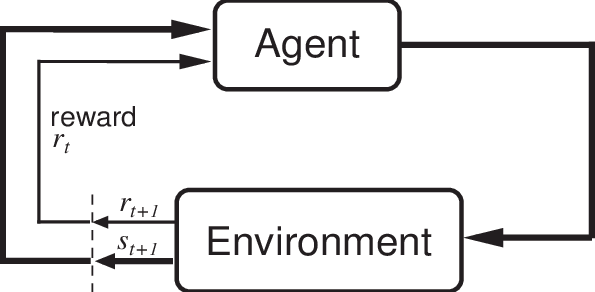
\includegraphics[width=10cm]{rl}
	\end{center}
	\caption{Figura: Idea generale di \textit{reinforcement learning}: un agente interagisce con l'ambiente per imparare dall'esperienza. Per ogni istante di tempo \textit{t} l'agente è in un certo stato \textit{S\textsubscript{t}} ed esegue l'azione \textit{A\textsubscript{t}}. Come risultato, passa in un nuovo stato \textit{S\textsubscript{t+1}} e riceve una ricompensa \textit{R\textsubscript{t+1}}}
\end{fig}

\\~\\Nel contesto di Sentyment il supervisore rappresenta l'agente che opera le scelte. L'ambiente (i dati in input) sono i dataset di qualche settimana che, a ogni iterazione del ciclo di scelta della nuova AI rappresentante, sono forniti all'algoritmo di reinforcement learning. La scelta che il supervisore deve operare ad ogni passo è decidere quale fra le dodici AI sta, secondo lui, agendo meglio delle altre; mentre l'output della scelta, ovvero la valutazione di efficacia, è il risultato di una funzione di score calcolata con indicatori statistici finanziari a partire dai trigger della AI scelta, il cui risultato viene confrontato con quello prodotto dalle altre AI competitori.

\subsection{Q-learning}


\subsection{Multi-armed bandit}
Un problema noto che si adatta alla situazione e fa uso di tecniche di reinforcement learning, implementato usando algoritmi di q-learning. La sua versione classica discosta leggermente da questo ambito ma può essere revisionato per trarre vantaggio dalla sua semplicità.\cite{rl}\\
Il problema originale illustra un contesto di gioco in cui.....

\newpage
\chapter{Risultati}
\label{cap5}

\newpage

%
%			BIBLIOGRAFIA
%
\begin{thebibliography}{9}
	\bibitem{es}
	Chalup, S., \& Maire, F. (1999, July). A study on hill climbing algorithms for neural network training. In Proceedings of the 1999 Congress on Evolutionary Computation-CEC99 (Cat. No. 99TH8406) (Vol. 3, pp. 2014-2021). IEEE.
	\bibitem{}
	Bengio, Y. (2009). Learning deep architectures for AI. Foundations and trends® in Machine Learning, 2(1), 1-127.
	\bibitem{}
	An, G. (1996). The effects of adding noise during backpropagation training on a generalization performance. Neural computation, 8(3), 643-674.
	\bibitem{aitest}
	Schmelzer, R. (2020, January 3). How Do You Test AI Systems?. Forbes. Last accessed 21th Feb 2020: https://www.forbes.com/sites/cognitiveworld/2020/01/03/how-do-you-test-ai-systems.
	\bibitem{rl}
	Sutton, R. S., \& Barto, A. G. (1998). Introduction to reinforcement learning (Vol. 135). Cambridge: MIT press.
	\bibitem{}
	Guijarro-Berdiñas, B., \& Alonso-Betanzos, A. (2002). Empirical evaluation of a hybrid intelligent monitoring system using different measures of effectiveness. Artificial Intelligence in Medicine, 24(1), 71-96.
\end{thebibliography}
\end{document}


 
